\chapter{Karbonil Terkonjugasi: Michael dan Robinson}\label{ch:b2:conjugate-additions}

Keempat cincin sebuah hormon steroid mula-mula dirakit satu cincin demi satu
cincin, dan satu urutan reaksi menjadi cara baku untuk menambahkan sebuah
cincin: urutan itu membangun satu cincin beranggota enam yang utuh, termasuk
ketonnya, dari sebuah keton dan sebuah keton tak jenuh yang kecil. Cara itu
berhasil karena gugus karbonil yang terkonjugasi dengan ikatan rangkap
\ce{C=C} meneruskan sifat elektrofiliknya ke ujung jauh ikatan rangkap itu.
Bab ini membahas ujung jauh itu: nukleofil mana yang menyerangnya, mengapa,
dan apa yang dapat dibangun dengannya.

\begin{recall}
\Cref{ch:b2:enolates-aldol}: \omterm{def:b2:enolates-aldol:enolate}{enolat}, \omterm{def:b2:enolates-aldol:aldol}{kondensasi aldol}. \Cref{ch:b2:frontier-orbitals}:
\omterm{def:b2:frontier-orbitals:control}{kendali muatan} dan \omterm{def:b2:frontier-orbitals:control}{kendali orbital}, pereaksi keras dan lunak.
\Cref{ch:b2:huckel}: orbital Hückel dan muatan $\pi$. Jilid Tahun 1: pereaksi
Grignard dan hidrida, kendali kinetik dan termodinamik, sistem terkonjugasi.
\end{recall}

\section{Dua situs elektrofilik}

\begin{definition}[Senyawa karbonil $\alpha,\beta$-tak jenuh]\label{def:b2:conjugate-additions:enone}
Sebuah \emph{senyawa karbonil $\alpha,\beta$-tak jenuh}\index{senyawa karbonil alfa,beta-tak jenuh@senyawa karbonil $\alpha,\beta$-tak jenuh}
mempunyai ikatan rangkap \ce{C=C} di antara karbon $\alpha$
dan $\beta$ sebuah senyawa karbonil, yang terkonjugasi dengan \ce{C=O}:
enon (keton), enal (aldehida), ester atau \omterm{def:b2:amines:nitrile}{nitril} tak jenuh. Yang paling
sederhana adalah propenal \ce{CH2=CHCHO} dan but-3-en-2-on \ce{CH2=CHCOCH3}
(metil vinil keton).
\end{definition}

\begin{omfigure}
\setchemfig{atom sep=1.9em}
\schemestart
\chemfig{H_2C=CH-CH=O}
\arrow{<->}
\chemfig{H_2C=CH-\chemabove{C}{\scriptstyle +}H-\chemabove{O}{\scriptstyle -}}
\arrow{<->}
\chemfig{\chemabove{C}{\scriptstyle +}H_2-CH=CH-\chemabove{O}{\scriptstyle -}}
\schemestop
\par\medskip

\begin{tikzpicture}
\begin{axis}[ybar, width=0.47\linewidth, height=4.6cm, ymin=-0.6, ymax=0.4,
  xtick={1,2,3,4}, xticklabels={C$\beta$,C$\alpha$,C(O),O}, axis x line=bottom, axis y line=left,
  extra y ticks={0}, extra y tick style={grid=major, grid style={black!50}}, enlarge x limits=0.15,
  tick label style={font=\scriptsize}, ylabel={muatan $\pi$}, label style={font=\small},
  title={\small muatan $\pi$ propenal}, bar width=8pt]
\addplot[fill=omDef!50, draw=omDef] table[x=atom, y=q] {figdata/out/bachelor-2-huckel-d.dat};
\end{axis}
\end{tikzpicture}\hfill
\begin{tikzpicture}
\begin{axis}[ybar, width=0.47\linewidth, height=4.6cm, ymin=-0.8, ymax=0.8,
  xtick={1,2,3,4}, xticklabels={C$\beta$,C$\alpha$,C(O),O}, axis x line=bottom, axis y line=left,
  extra y ticks={0}, extra y tick style={grid=major, grid style={black!50}}, enlarge x limits=0.15,
  tick label style={font=\scriptsize}, ylabel={koefisien}, label style={font=\small},
  title={\small LUMO propenal}, bar width=8pt]
\addplot[fill=omThm!45, draw=omThm] table[x=atom, y=c] {figdata/out/bachelor-2-huckel-d.dat};
\end{axis}
\end{tikzpicture}

{\small Propenal. Atas: ketiga struktur resonansinya; dua yang terakhir
menempatkan muatan positif pada karbon karbonil dan pada karbon $\beta$.
Bawah: model Hückel pada
\cref{ch:b2:frontier-orbitals} ($\alpha_{\ce{O}} = \alpha + \beta$, $\beta_{\ce{CO}} = \beta$; sebuah model).
Muatan positif terbesar terletak pada karbon karbonil (+0.33, dibandingkan
dengan +0.23 pada karbon $\beta$); koefisien \omterm{def:b2:frontier-orbitals:frontier}{LUMO} terbesar terletak pada
karbon $\beta$ (0.66, dibandingkan dengan $-0.58$).}
\end{omfigure}

\begin{proposition}[Dua situs]\label{prop:b2:conjugate-additions:two-sites}
Dalam senyawa karbonil $\alpha,\beta$-tak jenuh, karbon karbonil dan karbon
$\beta$ sama-sama elektrofilik. Karbon karbonil membawa muatan positif yang
lebih besar; karbon $\beta$ membawa koefisien yang lebih besar dalam \omterm{def:b2:frontier-orbitals:frontier}{LUMO}.
\end{proposition}

\begin{proof}[Argumen]
Struktur-struktur resonansi menempatkan muatan positif pada karbon karbonil
dan, melalui \ce{C=C}, pada karbon $\beta$; karbon $\alpha$ tidak pernah
positif. Model Hückel propenal membuat hal ini kuantitatif: menjumlahkan
$2c^2$ pada kedua orbital $\pi$ yang terisi menghasilkan muatan $\pi$
(\cref{def:b2:huckel:indices}) $+0.33$ pada karbon karbonil, $+0.23$ pada karbon $\beta$, $-0.03$
pada karbon $\alpha$, dan $-0.53$ pada oksigen. \omterm{def:b2:frontier-orbitals:frontier}{LUMO}, orbital yang menerima
elektron-elektron nukleofil, paling besar pada karbon $\beta$. Dengan
demikian, kedua situs itu menanggapi kedua jenis kendali pada
\cref{def:b2:frontier-orbitals:control}.
% figdata: bachelor-2/huckel.py part d
\end{proof}

\section{Adisi-1,2 atau adisi konjugat}

\begin{definition}[Cara adisi]\label{def:b2:conjugate-additions:addition-modes}
Nukleofil yang beradisi pada karbon karbonil sebuah senyawa karbonil
$\alpha,\beta$-tak jenuh menghasilkan
\emph{adisi-1,2}\index{adisi-1,2} (dihitung dari oksigen): sebuah alkoksida
alilik, lalu alkohol. Nukleofil yang beradisi pada karbon $\beta$
menghasilkan \emph{adisi konjugat}\index{adisi konjugat}
(atau adisi-1,4): sebuah \omterm{def:b2:enolates-aldol:enolate}{enolat}, yang terprotonasi pada karbon dan
menghasilkan senyawa karbonil jenuh yang tersubstitusi pada karbon $\beta$.
\end{definition}

\begin{omfigure}
\setchemfig{atom sep=1.9em}
\schemestart
\chemfig{*6(-=-(=O)---)}
\arrow{->[\ce{CH3Li}][lalu \ce{H2O}]}[,1.4]
\chemfig{*6(-=-(-[:75]CH_3)(-[:-15]OH)---)}
\schemestop
\hspace{2.5em}
\schemestart
\chemfig{*6(-=-(=O)---)}
\arrow{->[\ce{(CH3)2CuLi}][lalu \ce{H2O}]}[,1.6]
\chemfig{*6(-(-CH_3)--(=O)---)}
\schemestop
\par\vspace{6pt}

{\small Sikloheks-2-en-1-on dengan dua nukleofil metil. Metillitium, sebuah
\omterm{def:b2:frontier-orbitals:hard-soft}{nukleofil keras}, beradisi pada karbon karbonil: 1-metilsikloheks-2-en-1-ol
(\omterm{def:b2:conjugate-additions:addition-modes}{adisi-1,2}). Litium dimetilkuprat, sebuah \omterm{def:b2:frontier-orbitals:hard-soft}{nukleofil lunak}, beradisi pada
karbon $\beta$: 3-metilsikloheksanon (\omterm{def:b2:conjugate-additions:addition-modes}{adisi konjugat}).}
\end{omfigure}

\begin{proposition}[Situs yang mana]\label{prop:b2:conjugate-additions:regio}
\omterm{def:b2:frontier-orbitals:hard-soft}{Nukleofil keras} (organolitium, sebagian besar pereaksi Grignard, \ce{LiAlH4})
terutama beradisi 1,2, di bawah \omterm{def:b2:frontier-orbitals:control}{kendali muatan}, biasanya secara
ireversibel. \omterm{def:b2:frontier-orbitals:hard-soft}{Nukleofil lunak} (\omterm{def:b2:conjugate-additions:cuprate}{organokuprat}, \omterm{def:b2:enolates-aldol:enolate}{enolat} terstabilkan, tiolat,
amina) terutama beradisi 1,4, di bawah \omterm{def:b2:frontier-orbitals:control}{kendali orbital}; adduk konjugat, yang
mempertahankan ikatan \ce{C=O}, juga merupakan produk yang lebih stabil.
\end{proposition}

\begin{proof}[Argumen]
\omterm{def:b2:frontier-orbitals:hard-soft}{Nukleofil keras}, yang kecil dan bermuatan, berinteraksi terutama melalui
muatan: nukleofil itu menuju pusat yang paling positif, yaitu karbon
karbonil (\cref{prop:b2:conjugate-additions:two-sites}); adisinya cepat dan
tidak berbalik, sehingga produk-1,2, yang terbentuk lebih cepat, bertahan
(kendali kinetik). \omterm{def:b2:frontier-orbitals:hard-soft}{Nukleofil lunak}, yang besar dan mudah terpolarisasi,
dengan \omterm{def:b2:frontier-orbitals:frontier}{HOMO} yang tinggi, berinteraksi terutama melalui orbital-orbital
perbatasan: nukleofil itu menuju tempat \omterm{def:b2:frontier-orbitals:frontier}{LUMO} paling besar, yaitu karbon
$\beta$. Produk-1,4 mempertahankan ikatan $\pi$ \ce{C=O}, yang lebih kuat
daripada ikatan $\pi$ \ce{C=C} yang dipertahankan oleh produk-1,2; jika
adisi-adisinya reversibel (sianida, amina, \omterm{def:b2:enolates-aldol:enolate}{enolat} terstabilkan, alkoksida),
kesetimbangan karena itu bergeser ke adduk konjugat bahkan ketika
adduk-1,2 terbentuk lebih dahulu (kendali termodinamik).
\end{proof}

\begin{method}[Meramalkan cara adisi]\label{met:b2:conjugate-additions:predict-mode}
\begin{enumerate}
  \item Golongkan nukleofilnya: keras (\ce{RLi}, \ce{RMgX}, \ce{LiAlH4}, \ce{NaBH4} dengan aldehida)
        atau lunak (\ce{R2CuLi}, \omterm{def:b2:enolates-aldol:enolate}{enolat} 1,3-dikarbonil, \ce{RS-}, \ce{R2NH}, sianida pada kesetimbangan).
  \item Periksalah reversibilitasnya: adisi keras yang ireversibel
        menghasilkan produk-1,2; adisi yang reversibel, jika diberi waktu,
        menghasilkan produk-1,4.
  \item Periksalah halangannya: karbon $\beta$ yang tersubstitusi
        memperlambat adisi-1,4; aldehida, yang kurang terhalang dan lebih
        reaktif pada karbonilnya daripada keton, lebih menyukai 1,2.
  \item Tuliskan \omterm{def:b2:enolates-aldol:enolate}{enolat} yang terbentuk oleh adisi-1,4: \omterm{def:b2:enolates-aldol:enolate}{enolat} itu dapat
        diprotonasi, atau ditangkap oleh sebuah elektrofil.
\end{enumerate}
\end{method}

\section{Adisi Michael}

\begin{definition}[Adisi Michael]\label{def:b2:conjugate-additions:michael}
Yang disebut \emph{adisi Michael}\index{adisi Michael} adalah \omterm{def:b2:conjugate-additions:addition-modes}{adisi konjugat}
sebuah karbanion terstabilkan, biasanya \omterm{def:b2:enolates-aldol:enolate}{enolat}, pada senyawa karbonil
$\alpha,\beta$-tak jenuh atau alkena miskin elektron yang serupa.
Nukleofilnya adalah \emph{donor Michael}\index{donor Michael} (senyawa
1,3-dikarbonil, nitroalkana, sianoester); senyawa tak jenuhnya adalah
\emph{akseptor Michael}\index{akseptor Michael}
(enon, enal, ester tak jenuh, \omterm{def:b2:amines:nitrile}{nitril} tak jenuh, atau senyawa nitro tak jenuh).
\end{definition}

\begin{omfigure}
\setchemfig{atom sep=1.8em}
\schemestart
\chemfig{CH_2(-[:30]COOEt)(-[:-30]COOEt)}
\arrow{<=>[\ce{EtO-}][$-$ \ce{EtOH}]}[,1.3]
\chemfig{\chemabove{C}{\scriptstyle -}H(-[:30]COOEt)(-[:-30]COOEt)}
\+
\chemfig{H_2C=CH-C(=[2]O)-CH_3}
\schemestop

\medskip
\setchemfig{atom sep=1.6em}
\schemestart
\arrow{->[adisi]}[,0.95]
\chemfig{CH(-[:150]EtOOC)(-[:210]EtOOC)-CH_2-CH=C(-[2]\chemabove{O}{\scriptstyle -})-CH_3}
\arrow{->[\ce{EtOH}][$-$ \ce{EtO-}]}[,1.1]
\chemfig{CH(-[:150]EtOOC)(-[:210]EtOOC)-CH_2-CH_2-C(=[2]O)-CH_3}
\schemestop
\par\vspace{6pt}

{\small \omterm{def:b2:conjugate-additions:michael}{Adisi Michael} dietil propanadioat pada but-3-en-2-on. Etoksida
membentuk \omterm{def:b2:enolates-aldol:enolate}{enolat} yang terstabilkan; \omterm{def:b2:enolates-aldol:enolate}{enolat} itu beradisi pada karbon $\beta$;
\omterm{def:b2:enolates-aldol:enolate}{enolat} yang terbentuk mengambil proton dari etanol, yang meregenerasi
etoksida. Produknya, dietil (3-oksobutil)propanadioat, adalah senyawa
1,5-dikarbonil.}
\end{omfigure}

\begin{proposition}[Mekanisme Michael]\label{prop:b2:conjugate-additions:michael}
\omterm{def:b2:conjugate-additions:michael}{Adisi Michael} berlangsung dalam tiga tahap (deprotonasi donor, \omterm{def:b2:conjugate-additions:addition-modes}{adisi
konjugat}, protonasi \omterm{def:b2:enolates-aldol:enolate}{enolat} yang baru), dan basanya diregenerasi pada tahap
terakhir: jumlah katalitik sudah cukup.
\end{proposition}

\begin{proof}[Argumen]
Hidrogen $\alpha$ donor, yang terletak di antara dua karbonil, bersifat
asam: $\mathrm pK_a$ sekitar 13 untuk dietil
propanadioat, 10.7 untuk etil 3-oksobutanoat. Etoksida (etanol, 15.9)
melepaskannya dalam jumlah besar, yang lebih dari cukup. \omterm{def:b2:enolates-aldol:enolate}{Enolat} yang
terstabilkan dan lunak itu beradisi 1,4
(\cref{prop:b2:conjugate-additions:regio}). \omterm{def:b2:enolates-aldol:enolate}{Enolat} yang terbentuk adalah basa
yang lebih kuat daripada \omterm{def:b2:enolates-aldol:enolate}{enolat} donor (\omterm{def:b2:enolates-aldol:enolate}{enolat} itu distabilkan oleh satu
karbonil, bukan dua), sehingga mengambil proton dari pelarut dan
mengembalikan satu etoksida untuk setiap etoksida yang terpakai. Reaksi
keseluruhannya membentuk ikatan $\sigma$ \ce{C-C} dari ikatan $\pi$
\ce{C=C}: reaksi itu menguntungkan, dan dengan donor yang terstabilkan
adduknya tidak berbalik.
% ledger: pka:ethanol, pka:diethylmalonate, pka:acetoacetate
\end{proof}

Adduk Michael dengan keton di sisi donor dan keton di sisi akseptor adalah
senyawa 1,5-dikarbonil: kedua karbonil berjarak lima karbon, termasuk kedua
karbon karbonilnya. Pola itu adalah ciri khas \omterm{def:b2:conjugate-additions:michael}{adisi Michael}, seperti
senyawa $\beta$-hidroksi karbonil menjadi ciri khas \omterm{def:b2:enolates-aldol:aldol}{aldol}
(\cref{met:b2:enolates-aldol:aldol-recognition}).

\section{Organokuprat}

\begin{definition}[Organokuprat]\label{def:b2:conjugate-additions:cuprate}
Yang disebut \emph{organokuprat}\index{organokuprat} \ce{R2CuLi} adalah
senyawa tembaga(I) yang membawa dua gugus organik, dibuat dari dua
ekuivalen organolitium dan satu ekuivalen tembaga(I) halida:
\begin{equation*}
\ce{2 CH3Li + CuI -> (CH3)2CuLi + LiI}.
\end{equation*}
\end{definition}

\omterm{def:b2:conjugate-additions:cuprate}{Organokuprat} (disebut juga pereaksi Gilman) dibuat dan dipakai dalam eter
pada suhu rendah di bawah gas inert, seperti induk organolitiumnya. Tembaga
kurang elektropositif daripada litium atau magnesium, sehingga ikatan
\ce{Cu-C} lebih kovalen dan karbonnya kurang bermuatan: gugus metil sebuah
kuprat adalah \omterm{def:b2:frontier-orbitals:hard-soft}{nukleofil lunak}. Ada tiga kegunaannya.

\begin{itemize}
  \item \emph{\omterm{def:b2:conjugate-additions:addition-modes}{Adisi konjugat}} gugus alkil atau aril pada enon, yang tidak
        dapat dilakukan dengan bersih oleh pereaksi Grignard dan
        organolitium; hanya satu dari kedua gugus \ce{R} yang dipindahkan.
  \item \emph{Penangkapan}: \omterm{def:b2:enolates-aldol:enolate}{enolat} yang terbentuk oleh \omterm{def:b2:conjugate-additions:addition-modes}{adisi konjugat} dapat
        dialkilasi pada karbon $\alpha$-nya, sehingga dua ikatan \ce{C-C}
        baru terbentuk dalam satu operasi.
  \item \emph{Substitusi} halida: $\mathrm{R_2CuLi + R'Br \to R{-}R' + RCu + LiBr}$, sebuah
        kopling yang akan dirusak oleh organolitium melalui eliminasi atau
        pertukaran.
\end{itemize}

\section{Anulasi Robinson}

\begin{definition}[Anulasi]\label{def:b2:conjugate-additions:robinson}
Yang disebut \emph{anulasi}\index{anulasi} membangun cincin baru pada molekul
yang sudah ada. \emph{Anulasi Robinson}
\index{anulasi Robinson} membangun sikloheks-2-en-1-on: \omterm{def:b2:conjugate-additions:michael}{adisi Michael}
\omterm{def:b2:enolates-aldol:enolate}{enolat} sebuah keton pada keton $\alpha,\beta$-tak jenuh (biasanya
but-3-en-2-on), diikuti oleh \omterm{def:b2:enolates-aldol:aldol}{kondensasi aldol} intramolekular 1,5-diketon
yang terbentuk.
\end{definition}

\begin{omfigure}
\setchemfig{atom sep=1.8em}
\schemestart
\chemfig{[:30]*6(-(=O)-(-CH_3)-(=O)---)}
\+
\chemfig{=[:30]-[:-30](=[:-90]O)-[:30]}
\arrow{->[basa][Michael]}[,1.2]
\chemfig{[:30]*6(-(=O)-(-[:40]CH_3)(-[:-30]-[:30]-[:-30](=[:-90]O)-[:30])-(=O)---)}
\schemestop

\medskip
\schemestart
\arrow{->[basa][aldol]}[,1.1]
\chemfig{[:-30]*6(---(-[:-60]OH)*6(--(=O)---)-(-[:105]CH_3)-(=O)-)}
\arrow{->[panas][$-$ \ce{H2O}]}[,1.1]
\chemfig{[:-30]*6(---*6(=-(=O)---)-(-[:105]CH_3)-(=O)-)}
\schemestop
\par\vspace{6pt}

{\small \omterm{def:b2:conjugate-additions:robinson}{Anulasi Robinson} yang menghasilkan keton Wieland--Miescher. \omterm{def:b2:enolates-aldol:enolate}{Enolat}
2-metilsikloheksana-1,3-dion beradisi pada but-3-en-2-on (Michael): sebuah
triketon. \omterm{def:b2:enolates-aldol:enolate}{Enolat} dari metil keton pada rantai samping menyerang sebuah
karbonil cincin (\omterm{def:b2:enolates-aldol:aldol}{aldol} intramolekular), sehingga menutup cincin beranggota enam; dehidrasi
menghasilkan enon terkonjugasi. Gugus metil angular berada pada karbon yang
dipakai bersama oleh kedua cincin, satu-satunya pusat stereogenik.}
\end{omfigure}

\begin{proposition}[Anulasi Robinson]\label{prop:b2:conjugate-additions:robinson}
Keton dengan hidrogen $\alpha$ dan but-3-en-2-on, dalam basa, menghasilkan
sikloheks-2-en-1-on dalam tiga tahap: \omterm{def:b2:conjugate-additions:michael}{adisi Michael}, \omterm{def:b2:enolates-aldol:aldol}{adisi aldol}
intramolekular yang membentuk cincin beranggota enam, dan dehidrasi. Cincin
yang baru mengandung bekas karbon $\alpha$ keton dan karbon karbonilnya,
serta keempat karbon but-3-en-2-on.
\end{proposition}

\begin{proof}
Ikutilah atom-atomnya pada gambar. Karbon \omterm{def:b2:enolates-aldol:enolate}{enolat} keton (sebut saja
C$_a$) berikatan dengan karbon $\beta$
but-3-en-2-on: rantai C$_a$--\ce{CH2}--\ce{CH2}--\ce{C(=O)}--\ce{CH3} tergantung pada C$_a$, dan
C$_a$ masih terikat pada karbon karbonil keton C$_k$. Dalam basa, metil
keton rantai itu membentuk \omterm{def:b2:enolates-aldol:enolate}{enolatnya} pada \ce{CH3} ujung, yang menyerang
C$_k$. Cincin yang tertutup terdiri atas C$_k$, C$_a$,
kedua \ce{CH2}, karbon karbonil rantai samping, dan bekas karbon metil:
enam atom, ukuran cincin yang bebas tegangan, itulah sebabnya \omterm{def:b2:enolates-aldol:enolate}{enolat} ini, di
antara \omterm{def:b2:enolates-aldol:enolate}{enolat-enolat} yang mungkin, menghasilkan produk yang stabil (serangan
oleh \omterm{def:b2:enolates-aldol:enolate}{enolat} \ce{CH2} bagian dalam rantai akan menutup cincin beranggota
empat). \omterm{def:b2:enolates-aldol:aldol}{Aldolnya} mempunyai
\ce{OH} pada C$_k$, $\beta$ terhadap karbonil rantai; dehidrasi menempatkan
\ce{C=C} di antara C$_k$ dan bekas karbon metil, terkonjugasi dengan
karbonil: sebuah sikloheks-2-en-1-on.
\end{proof}

\begin{method}[Memutus sebuah sikloheksenon]\label{met:b2:conjugate-additions:robinson-disconnection}
\begin{enumerate}
  \item Temukan sikloheks-2-en-1-on dalam target; beri nomor karbon
        karbonilnya C1, ikatan rangkapnya C2=C3, dan cincinnya terus sampai C6.
  \item Batalkan dehidrasinya: sebuah \ce{OH} pada C3, sebuah \ce{C-H} pada C2.
  \item Batalkan \omterm{def:b2:enolates-aldol:aldol}{aldolnya}: potong C2--C3. C3 menjadi karbonil keton, C2
        menjadi gugus metil sebuah metil keton: sebuah 1,5-diketon.
  \item Batalkan \omterm{def:b2:conjugate-additions:michael}{adisi Michael-nya}: potong ikatan antara C4 (karbon
        $\alpha$ keton C3) dan C5. Donornya adalah keton itu; akseptornya
        adalah enon C5=C6--C1(=O)--C2, yang merupakan but-3-en-2-on jika C5,
        C6, dan C2 hanya membawa hidrogen.
\end{enumerate}
\end{method}

\begin{history}[Anulasi, 1935]
\begin{minipage}[t]{0.18\linewidth}
\vspace{0pt}
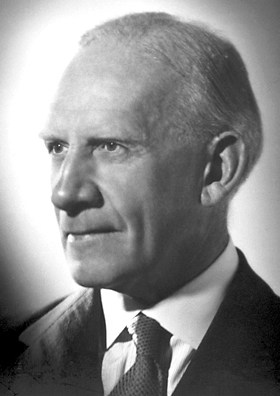
\includegraphics[width=\linewidth]{images/book3/robinson.jpg}
\end{minipage}\hfill
\begin{minipage}[t]{0.78\linewidth}
\vspace{0pt}
Robert Robinson dan William Rapson menerbitkan urutan pembentuk cincin itu
pada tahun 1935, dalam penelitian yang ditujukan pada sintesis steroid.
Pencapaian utama Robinson adalah struktur dan sintesis alkaloid, yang
membuatnya menerima Hadiah Nobel Kimia 1947. Pada tahun 1950 Peter Wieland
dan Karl Miescher membuat diketon bisiklik pada soal bab ini, yang menjadi
titik awal yang lazim bagi sintesis steroid dan terpena. (Potret: pembuat
tidak diketahui, domain publik; Wikimedia Commons.)
\end{minipage}
\end{history}

\begin{safety}{\ghs[5mm]{GHS02}\,\ghs[5mm]{GHS05}\,\ghs[5mm]{GHS06}\,\ghs[5mm]{GHS07}\,\ghs[5mm]{GHS08}\,\ghs[5mm]{GHS09}}
But-3-en-2-on mudah terbakar, sangat beracun, korosif, dan berbahaya bagi
lingkungan akuatik, serta merupakan lakrimator yang kuat; senyawa ini hanya
ditangani di dalam lemari asam. Sikloheks-2-en-1-on mudah terbakar dan
beracun. Organolitium, pereaksi Grignard, dan kuprat bereaksi hebat dengan
air dan ditangani di bawah gas inert.
% ledger: ghs:MVK, ghs:cyclohexenone, ghs:MeMgBr
\end{safety}

\section{Latihan}

\begin{exercise}[$\star$]\label{exo:b2:conjugate-additions:1}
Ramalkan \omterm{def:b2:conjugate-additions:addition-modes}{adisi-1,2} atau adisi-1,4 pada sikloheks-2-en-1-on untuk:
\ce{CH3MgBr}; \ce{(CH3)2CuLi}; \ce{C6H5SH} dengan sedikit basa; \ce{LiAlH4}.
\end{exercise}

\begin{exercise}[$\star$]\label{exo:b2:conjugate-additions:2}
Golongkan sebagai \omterm{def:b2:conjugate-additions:michael}{donor Michael} atau \omterm{def:b2:conjugate-additions:michael}{akseptor Michael}: pentana-2,4-dion,
propenanitril \ce{CH2=CHCN}, nitrometana, metil propenoat, dietil
propanadioat, but-3-en-2-on.
\end{exercise}

\begin{exercise}[$\star$]\label{exo:b2:conjugate-additions:3}
Tuliskan pembuatan litium dibutilkuprat dari 1-bromobutana, litium, dan tembaga(I) iodida.
\end{exercise}

\begin{exercise}[$\star$]\label{exo:b2:conjugate-additions:4}
Tuliskan produk dietil propanadioat dengan but-3-en-2-on dan natrium
etoksida dalam jumlah katalitik, lalu produknya setelah hidrolisis dan
pemanasan.
\end{exercise}

\begin{exercise}[$\star\star$]\label{exo:b2:conjugate-additions:5}
Usulkan pembuatan 3-metilsikloheksanon dari sikloheks-2-en-1-on, dan
jelaskan mengapa metilmagnesium bromida merupakan pilihan yang buruk.
\end{exercise}

\begin{exercise}[$\star\star$]\label{exo:b2:conjugate-additions:6}
Etanatiol beradisi pada but-3-en-2-on dengan sekelumit trietilamina.
Tuliskan mekanismenya dan jelaskan mengapa tiolat beradisi 1,4.
\end{exercise}

\begin{exercise}[$\star\star$]\label{exo:b2:conjugate-additions:7}
Sianida dengan sikloheks-2-en-1-on menghasilkan, pada suhu rendah dan waktu
singkat, sianohidrin; pada suhu lebih tinggi dan waktu lebih lama,
3-oksosikloheksana-1-karbonitril. Jelaskan dengan kendali kinetik dan
termodinamik.
\end{exercise}

\begin{exercise}[$\star\star$]\label{exo:b2:conjugate-additions:8}
Tuliskan produk \omterm{def:b2:conjugate-additions:robinson}{anulasi Robinson} 2-metilsikloheksana-1,3-dion dengan
but-3-en-2-on, lalu produk sikloheksanon dengan but-3-en-2-on.
\end{exercise}

\begin{exercise}[$\star\star$]\label{exo:b2:conjugate-additions:9}
Putuskan heptana-2,6-dion menjadi \omterm{def:b2:conjugate-additions:michael}{donor Michael} dan \omterm{def:b2:conjugate-additions:michael}{akseptor Michael}, dan usulkan kondisinya.
\end{exercise}

\begin{exercise}[$\star\star\star$]\label{exo:b2:conjugate-additions:10}
\omterm{def:b2:enolates-aldol:aldol}{Adisi aldol} sederhana mudah berbalik dalam basa; adduk Michael dietil
propanadioat dan but-3-en-2-on tidak. Jelaskan dengan ikatan-ikatan yang
terbentuk dan terputus serta dengan keasaman produknya.
\end{exercise}

\begin{exercise}[$\star\star\star$]\label{exo:b2:conjugate-additions:11}
Dietil propanadioat dengan dua ekuivalen metil propenoat dan basa katalitik
menghasilkan produk yang tidak lagi mempunyai \ce{C-H} di antara kedua gugus
esternya. Gambarlah produk itu dan jelaskan.
\end{exercise}

\begin{exercise}[$\star\star\star$]\label{exo:b2:conjugate-additions:12}
2-Metilsikloheksanon dan but-3-en-2-on dalam \omterm{def:b2:conjugate-additions:robinson}{anulasi Robinson} dapat bereaksi
melalui salah satu dari kedua \omterm{def:b2:enolates-aldol:enolate}{enolat}. Gambarlah kedua produknya dan
nyatakan kondisi mana yang lebih menghasilkan produk dengan gugus metil
pada karbon fusi cincin.
\end{exercise}

\clearpage
\enlargethispage{3\baselineskip}
\section{Soal: Keton Wieland--Miescher}

\begin{problem}[{Soal akhir pekan --- donor yang asam, adduk Michael, aldol
intramolekular dan dehidrasinya, pusat stereogenik, dan neraca massa sebuah
preparasi}]
\label{pb:b2:conjugate-additions:1}
Preparasi (data latihan): \qty{10.0}{g} 2-metilsikloheksana-1,3-dion
direaksikan dengan sedikit kelebihan but-3-en-2-on dan basa katalitik
(\omterm{def:b2:conjugate-additions:michael}{adisi Michael}); triketonnya lalu disiklisasi dengan \omterm{def:b2:amines:class}{amina sekunder} dan
sebuah asam (\omterm{def:b2:enolates-aldol:aldol}{aldol}, dehidrasi). Rendemen keseluruhan: 70~\%. Senyawa induk
sikloheksana-1,3-dion mempunyai $\mathrm pK_a = 5.3$ dalam air. Massa molar
(\unit{g/mol}): C 12.011, H 1.008, O 15.999.
% ledger: pka:cyclohexanedione, aw:C, aw:H, aw:O, ghs:methylcyclohexanedione, ghs:MVK

\medskip
\noindent\textbf{Bagian I --- Donor.}
\begin{enumerate}
  \item Gambarlah 2-metilsikloheksana-1,3-dion dan tandailah hidrogennya yang paling asam.
  \item Mengapa hidrogen itu jauh lebih asam daripada hidrogen-hidrogen $\alpha$ sikloheksanon?
  \item Gambarlah ketiga struktur resonansi \omterm{def:b2:enolates-aldol:enolate}{enolatnya}.
  \item Apakah hidroksida atau etoksida cukup kuat untuk membentuk \omterm{def:b2:enolates-aldol:enolate}{enolat}
        ini secara lengkap? Gunakan $\mathrm pK_a$.
  \item Tuliskan \omterm{def:b2:enolates-aldol:tautomerism}{enol} dion itu yang melibatkan C2, dan jelaskan mengapa
        gugus metil pada C2 tidak mencegahnya.
  \item Apakah \omterm{def:b2:enolates-aldol:enolate}{enolat} ini keras atau lunak? Situs but-3-en-2-on manakah
        yang akan diserangnya?
\end{enumerate}

\medskip
\noindent\textbf{Bagian II --- Adduk Michael.}
\begin{enumerate}[resume]
  \item Tuliskan \omterm{def:b2:conjugate-additions:michael}{adisi Michael-nya} dan namailah triketon yang terbentuk.
  \item Mengapa hanya diperlukan basa dalam jumlah katalitik?
  \item Mengapa ikatan baru terbentuk pada C2 dion alih-alih pada oksigennya?
  \item Berapa karbon kuaterner yang dimiliki triketon itu?
  \item Kenalilah hubungan 1,5-dikarbonil dalam triketon itu.
  \item Mengapa dipakai sedikit kelebihan but-3-en-2-on, dan mengapa hanya sedikit?
\end{enumerate}

\medskip
\noindent\textbf{Bagian III --- Penutupan cincin.}
\begin{enumerate}[resume]
  \item Daftarlah karbon-karbon triketon yang membawa hidrogen $\alpha$.
  \item \omterm{def:b2:enolates-aldol:enolate}{Enolat} manakah, yang menyerang karbonil mana, yang menutup cincin beranggota enam?
  \item Penutupan cincin lain apa yang dapat dicoba, dan mengapa penutupan
        itu tidak menghasilkan produk?
  \item Tuliskan \omterm{def:b2:enolates-aldol:aldol}{aldol} yang terbentuk dan dehidrasi yang menyusulnya.
  \item Mengapa dehidrasinya mudah?
  \item Sebutkan gugus-gugus fungsi keton Wieland--Miescher.
\end{enumerate}

\medskip
\noindent\textbf{Bagian IV --- Stereokimia dan neraca massa.}
\begin{enumerate}[resume]
  \item Karbon manakah dalam produk yang merupakan pusat stereogenik?
  \item Apakah produk preparasi ini aktif secara optik? Jelaskan.
  \item Hitunglah massa molar dion, but-3-en-2-on, dan produk
        \ce{C11H14O2}.
  \item Tuliskan persamaan keseluruhannya dan periksalah dengan rumus-rumusnya.
  \item Hitunglah jumlah dion yang dipakai.
  \item Nyatakan massa keton Wieland--Miescher yang diperoleh pada rendemen
        keseluruhan 70~\%.
\end{enumerate}
\end{problem}
